\section{Do you consider your childhood to have been a happy one?}
Yes, I do consider my childhood to have been a happy one.
There was almost always someone to play with.
The big farm house had four porches, one on each side of the house.
So we could each claim a porch and there we would set up housekeeping with our dolls.
We could then make visits to the other households.
There was a small shed that had rabbit cages in it.
For a while we were allowed to clean it up and set up a school room.
I enjoyed getting the school set up but once that was complete playing school did not seem to be as much fun.
There were also times when Mimi and Wilmer, our cousins joined us to play.
%Image #7 With cousins and dolls
\begin{figure}
\centering
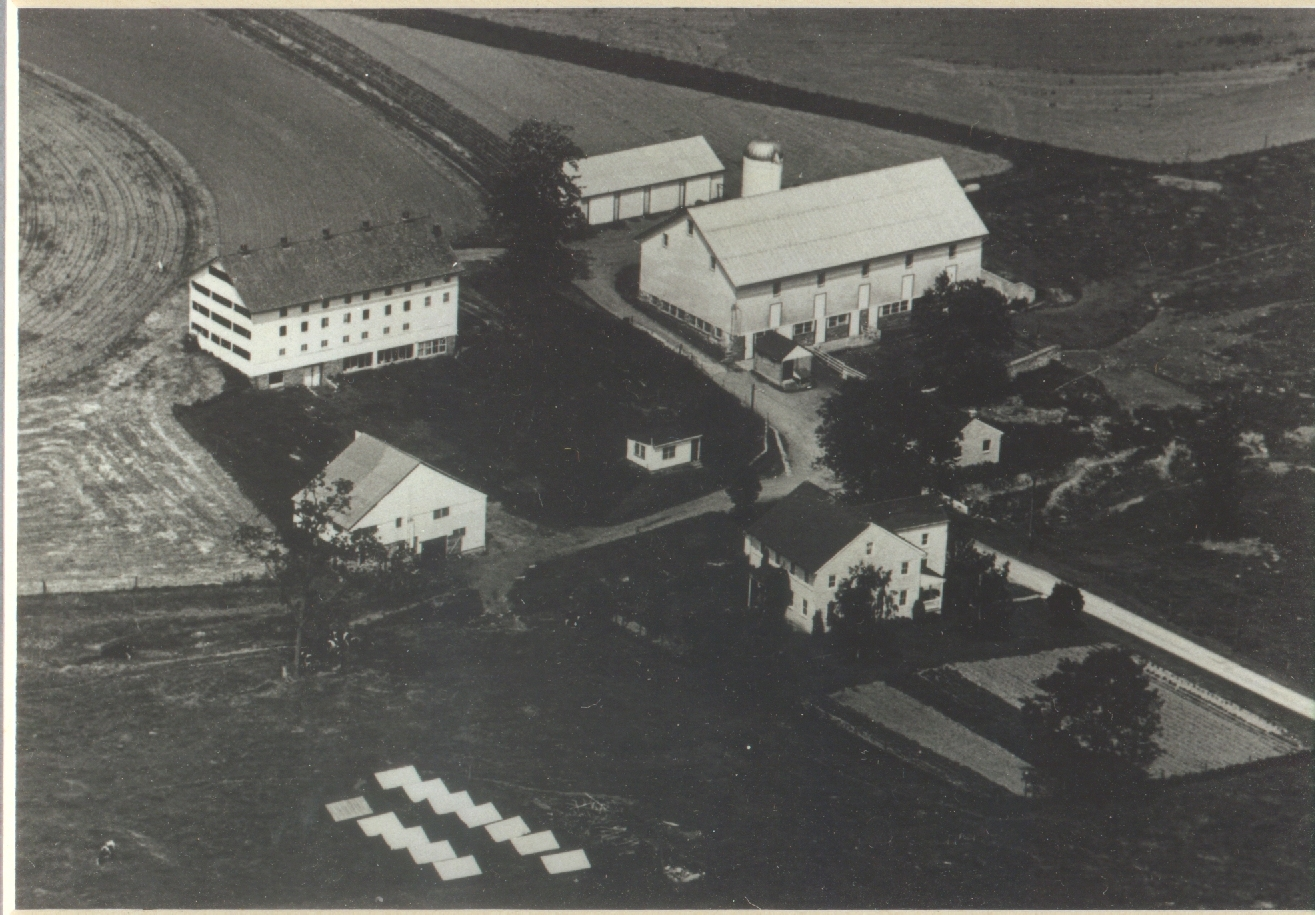
\includegraphics[width=0.75\textwidth]{childhood/7.jpg}
\caption{
Cousins and dolls.
}
\end{figure}


There were the older siblings to follow after when they went to the haymow and built tunnels with the bales.
During the spring my mother would take us to the woods and we would find wild flowers.
When we were more adventurous we might hike to a small cave in the hillside above the Conestoga River.
It is thought that Native Americans (the Conestoga Indians) used the cave as a place to overnight when traveling along the Conestoga River.
%Image #5 In the woods
\begin{figure}
\centering
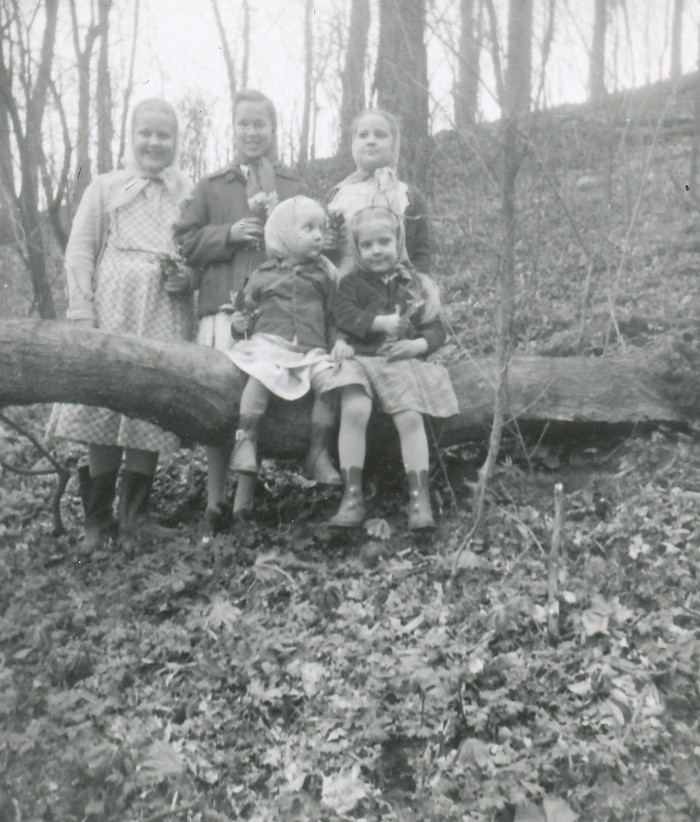
\includegraphics[width=0.75\textwidth]{childhood/5.jpg}
\caption{
In the woods.
}
\end{figure}

There were summer jobs such as shelling peas and later lima beans by the bucketsful.
There were stories to tell and guessing games to play while we did this.
It was special when Papa came and helped with the shelling.
He sat on the big green Adirondack chair and his big hands seemed to empty the baskets so much more quickly than when it was just the children shelling.

I remember having the job of cutting the asparagus.
The patch was a large section of the garden and I remember not liking to do this barefooted because of the sharp stones that hurt my feet.
I was glad when we stopped cutting asparagus toward the end of June.

Summer evenings after a game of beckon we lined up on the basement step to take our turn washing our feet and then it was off to bed.
%Image #6 Playing washing laundry
\begin{figure}
\centering
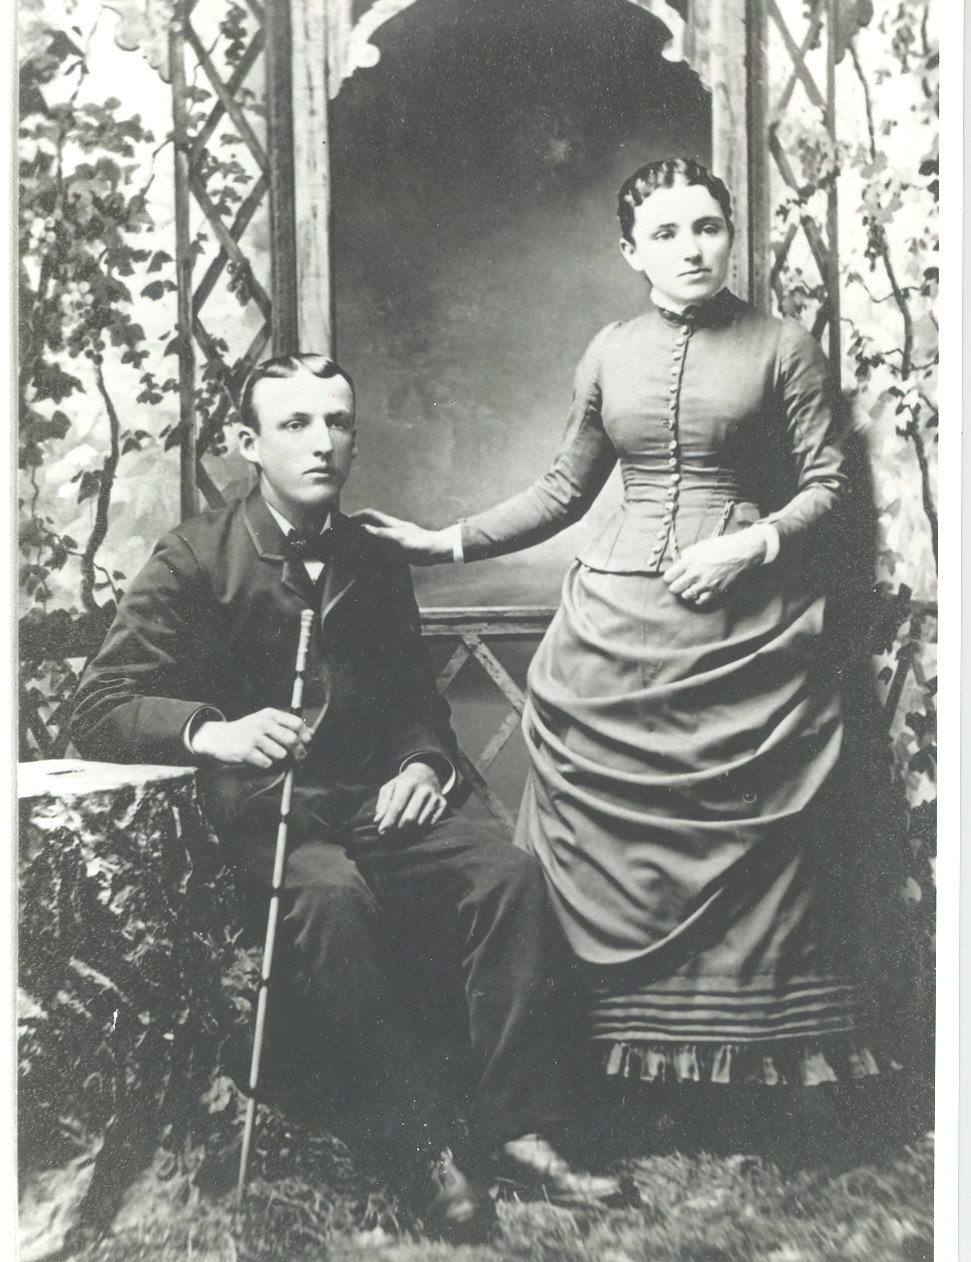
\includegraphics[width=0.8\textwidth]{childhood/6.jpg}
\caption{
Playing and washing laundry.
}
\end{figure}

On holidays there were usually extended family gatherings.
Christmas was held at Aunties.
Easter, I'm not sure where.
The Fourth of July was a picnic and watching the Lancaster fireworks from Auntie's back acreage.
I can remember that as the sun set, the grass cooled my bare feet.
I found a spot on a blanket or lawn chair then we waited for the first blossom of fireworks to explode above the horizon.
After minutes of oohing and awing there came the finally of multiple colors and many booms.
Then we packed into the station wagon and some of us may have fallen asleep before we reached the farm.
%Image #7.5 Cousin line up at Thanksgiving
Thanksgiving was most often hosted by my mother at our farm.
These gathering were my mother's siblings and their families.
If everyone attended that would be 11 adults and 28 children.
Uncle Marvin and his family lived in Arizona and so did not attend very often.
Some gathering included my mother's cousins and their families.
%Image #1 Family photo taken at Aunties in the early 60s
\begin{figure}
\centering
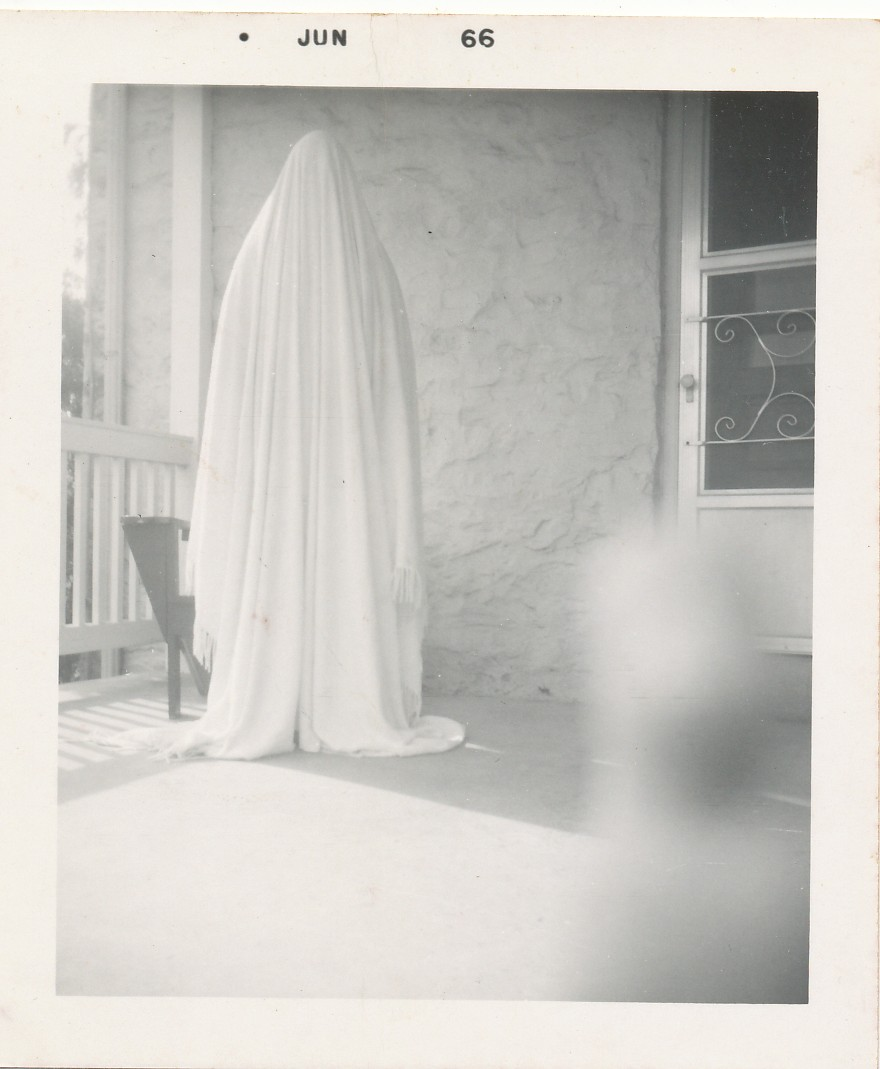
\includegraphics[width=1.0\textwidth]{childhood/1.jpg}
\caption{
Family photo taken at Aunties in the early 60s
}
\end{figure}

At home among the children there were squabbles and fights that occasionally got physical but these were the people that I had in my life so we most often got along.
We were expected to be kind to each other so slapping was severely frowned upon.
Did I love my family? I'm not sure I would have thought to articulate my understanding in that way.
But this was my family.
What else did I know?

